\hypertarget{chapter-1}{%
\section{Chapter 1}\label{chapter-1}}

In-text references to Figure \ref{fig:1}B and Table \ref{tab:foobar}
results in \textbf{Figure 1B and Table 1}.

Multi-reference to Figures \ref{fig:1} (A), the cool part of
\ref{fig:1} \& \ref{fig:three} and Tables \ref{tab:foobar} (very
cool) \& \emph{especially} \ref{tab:foobar} is rendered as
\textbf{Figures 1 (A), the cool part of 1 \& 2 and Tables 1 (verycool)
\& \emph{especially} 1}

\begin{figure}
\hypertarget{fig:1}{%
\centering
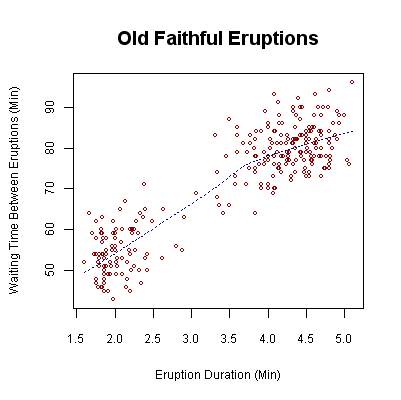
\includegraphics[width=1in,height=\textheight]{img/fig-1.png}
\caption{Figure 1: The number one.}\label{fig:1}
}
\end{figure}

\begin{figure}
\hypertarget{fig:}{%
\centering
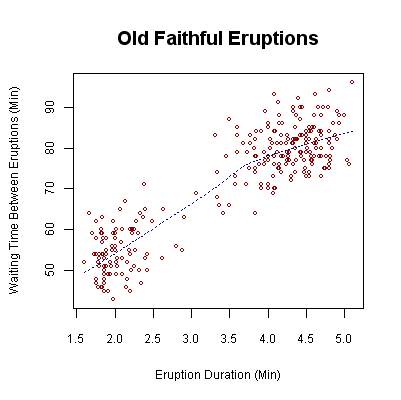
\includegraphics[width=1in,height=\textheight]{img/fig-1.png}
\caption{Figure 2: The unlabeled number two.}\label{fig:}
}
\end{figure}

\begin{figure}
\hypertarget{fig:three}{%
\centering
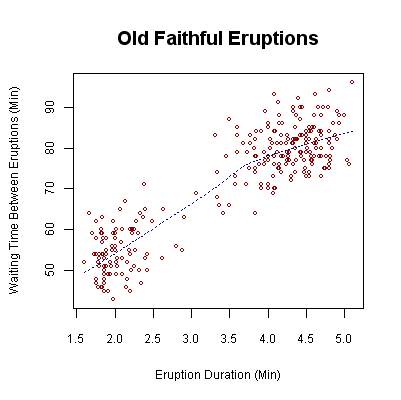
\includegraphics[width=1in,height=\textheight]{img/fig-1.png}
\caption{Figure 3: The number three.}\label{fig:three}
}
\end{figure}

Plot \ref{fig:three} is given above, without adding the ``Figure''
prefix.

As seen in Table \ref{tab:foobar}, commas are handled properly.

\hypertarget{equationchapter}{%
\subsection{Equations}\label{equationchapter}}

Equations, such as Equation \ref{eq:pythagoras}, have to be put into a
span with an id:

$$\label{eq:pythagoras}a^2 + b^2 = c^2$$

\hypertarget{tables}{%
\subsection{Tables}\label{tables}}

\begin{longtable}[]{@{}ll@{}}
\caption{Caption\label{tab:foobar}}\tabularnewline
\toprule
Foo & Bar \\
\midrule
\endfirsthead
\toprule
Foo & Bar \\
\midrule
\endhead
1 & 2 \\
\bottomrule
\end{longtable}

\hypertarget{another-chapter}{%
\section{Another chapter}\label{another-chapter}}

References to Section \ref{equationchapter} and the unnamed
Section \ref{another-chapter}

Text at end.
